\documentclass[aspectratio=169]{beamer}

% Theme and Color Scheme
\usetheme{Madrid}
\usecolortheme{beaver}

% Packages
\usepackage[utf8]{inputenc}
\usepackage{graphicx}
\usepackage{tikz}
\usepackage{fontawesome5}
\usepackage{xcolor}
\usepackage{amsmath}
\usepackage{array}

% Custom Colors
\definecolor{myNewColorA}{RGB}{206,008,20}
\definecolor{myNewColorB}{RGB}{26,168,217}
\definecolor{myNewColorC}{RGB}{245, 233, 85}
\definecolor{darkblue}{RGB}{0,51,102}
\definecolor{lightblue}{RGB}{173,216,230}

\setbeamercolor*{palette primary}{bg=myNewColorC}
\setbeamercolor*{palette secondary}{bg=myNewColorB, fg=white}
\setbeamercolor*{palette tertiary}{bg=myNewColorA, fg=white}
\setbeamercolor*{titlelike}{fg=myNewColorA}
\setbeamercolor*{title}{bg=myNewColorA, fg=white}
\setbeamercolor*{item}{fg=myNewColorA}
\setbeamercolor*{caption name}{fg=myNewColorA}
\usefonttheme{professionalfonts}
\usepackage{natbib}
\usepackage{hyperref}

% Title Information
\titlegraphic{
\includegraphics[height=1.5cm]{UNESWA_logo.png}}

\setbeamerfont{title}{size=\large}
\setbeamerfont{subtitle}{size=\small}
\setbeamerfont{author}{size=\small}
\setbeamerfont{date}{size=\small}
\setbeamerfont{institute}{size=\small}

\title[University of Eswatini]{Introduction to Computer Science}
\subtitle{CSC111 - Unit 7: Systems Analysis and Design}
\author[J.S.D]{Mr. Johnson Dlamini}
\institute[jsdlamini@uniswa.sz]{The University of Eswatini}
\date{\today}

\AtBeginSection[]{
  \begin{frame}
  \vfill
  \centering
  \begin{beamercolorbox}[sep=8pt,center,shadow=true,rounded=true]{title}
    \usebeamerfont{title}\insertsectionhead\par%
  \end{beamercolorbox}
  \vfill
  \end{frame}
}

\begin{document}

% Title Slide
\frame{\titlepage}

% Table of Contents
\begin{frame}{Outline}
    \tableofcontents
\end{frame}

% Section 1: Introduction
\section{Introduction}

\begin{frame}{Unit Overview}
    \begin{columns}
        \begin{column}{0.6\textwidth}
            \textbf{What we'll explore:}
            \begin{itemize}
                \item System definition and development
                \item Key elements of a system
                \item System Development Life Cycle (SDLC)
                \item Phases of system development
                \item Why systems fail
                \item System documentation
            \end{itemize}
        \end{column}
        \begin{column}{0.4\textwidth}
            \centering
            \faLaptopCode
            
            \vspace{1cm}
            {\Large \faCogs}
            
            \small{\textit{Systems Analysis \& Design}}
        \end{column}
    \end{columns}
    
    \vspace{0.5cm}
    \begin{alertblock}{Learning Focus}
        Understanding the principles of systems analysis, design, and development methodologies.
    \end{alertblock}
\end{frame}

\begin{frame}{Learning Outcomes}
    \textbf{After studying this unit, you should be able to:}
    \begin{enumerate}
        \item  Define a system
        \item  Describe a system development life cycle (SDLC)
        \item  Outline elements of a system
        \item  Explain the phases of SDLC
        \item  Explain why systems fail
        \item  Explain areas of system to be documented
        \item  Explain why system should be documented
    \end{enumerate}
    
    \vspace{0.3cm}
    \begin{exampleblock}{Key Concepts}
        We'll examine how organizations plan, build, and maintain information systems effectively.
    \end{exampleblock}
\end{frame}

% Section 2: System Definition
\section{System Definition}

\begin{frame}{What is a System?}
    \begin{definition}
        A \textbf{system} is defined as a collection of related subsystems or components that interact to perform a task in order to accomplish a goal.
    \end{definition}
    
    \vspace{0.3cm}
    \textbf{Computer-Based Information System Components:}
    \begin{itemize}
        \item   Hardware
        \item  Software
        \item  Data
        \item   Information
        \item   People
        \item   Communications setups
    \end{itemize}
    
    \vspace{0.2cm}
    \begin{exampleblock}{Application}
        Any organization that uses information technology will utilize a computer-based information system consisting of these components.
    \end{exampleblock}
\end{frame}

\begin{frame}{System Development}
    \textbf{Two Main Components:}
    
    \begin{columns}
        \begin{column}{0.48\textwidth}
            \begin{block}{◆\, Systems Analysis}
                \begin{itemize}
                    \item Gathering and interpreting facts
                    \item Diagnosing problems
                    \item Recommending improvements
                    \item Understanding the old system
                    \item Determining computer effectiveness
                \end{itemize}
            \end{block}
        \end{column}
        \begin{column}{0.48\textwidth}
            \begin{block}{◆\, Systems Design}
                \begin{itemize}
                    \item Planning new business systems
                    \item Complementing existing systems
                    \item Implementing solutions
                    \item Making systems better
                \end{itemize}
            \end{block}
        \end{column}
    \end{columns}
    
    \vspace{0.5cm}
    \begin{alertblock}{Systems Approach}
        The point of systems analysis and design is to ascertain how a system works and then take steps to make it better.
    \end{alertblock}
\end{frame}

\begin{frame}{When Organizations Need Change}
    \textbf{Organizations need to change their information systems in response to:}
    
    \begin{itemize}
        \item\, New marketing opportunities
        \item\, Modified government regulations
        \item\, Introduction of new technology
        \item\, Merger with another company
        \item\, Competitive pressures
        \item\, Performance issues
    \end{itemize}
    
    \vspace{0.5cm}
    \begin{exampleblock}{The Right Time}
        When change is needed, the time is ripe for applying the principles of systems analysis and design.
    \end{exampleblock}
\end{frame}

% Section 3: Elements of a System
\section{Elements of a System}

\begin{frame}{Key Elements of a System}
    \textbf{Six Key Elements to Consider:}


     \begin{columns}
        \begin{column}{0.48\textwidth}
          \begin{enumerate}
        \item[1.] \faArrowRight\, \textbf{Inputs and Outputs } 
   
        \item[2.] \faCog\, \textbf{Processor(s)}
      
        
        \item[3.] \faGamepad\, \textbf{Control}

 

         
    \end{enumerate}
    
        \end{column}
            \begin{column}{0.48\textwidth}
              \begin{enumerate} 

          \item[4.] \faRetweet\, \textbf{Feedback}
    
        \item[5.] \faGlobe\, \textbf{Environment} 
        \item[6.] \faDrawPolygon\, \textbf{Boundaries and Interface}

         
    \end{enumerate}
        \end{column}

        \end{columns}
    
\end{frame}

 

\begin{frame}{Outputs and Inputs}
    \begin{columns}
        \begin{column}{0.48\textwidth}
            \begin{block}{\faFileExport\, Outputs}
                \begin{itemize}
                    \item Main goal of the system
                    \item Produce value to users
                    \item Goods, services, or information
                    \item Must meet user expectations
                \end{itemize}
            \end{block}
        \end{column}
        \begin{column}{0.48\textwidth}
            \begin{block}{\faFileExport\, Inputs}
                \begin{itemize}
                    \item Material resources
                    \item Human resources
                    \item Information
                    \item Enter system for processing
                \end{itemize}
            \end{block}
        \end{column}
    \end{columns}
    
    \vspace{0.5cm}
    \begin{center}
        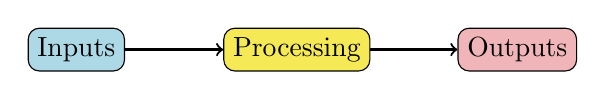
\begin{tikzpicture}[scale=0.8]
            \node[draw, fill=lightblue, rounded corners] (input) at (0,0) {Inputs};
            \node[draw, fill=myNewColorC, rounded corners] (process) at (3.5,0) {Processing};
            \node[draw, fill=myNewColorA!30, rounded corners] (output) at (7,0) {Outputs};
            \draw[->, thick] (input) -- (process);
            \draw[->, thick] (process) -- (output);
        \end{tikzpicture}
    \end{center}
    
    \begin{exampleblock}{First Step}
        Determining the output is a first step in specifying the nature, amount, and regularity of the input needed to operate a system.
    \end{exampleblock}
\end{frame}

\begin{frame}{Processor(s)}
    \begin{definition}
        The \textbf{processor} is the element of a system that involves the actual transformation of input into output.
    \end{definition}
    
    \vspace{0.5cm}
    \textbf{Key Characteristics:}
    \begin{itemize}
        \item   Operational component of a system
        \item  Transforms input into output
        \item  May modify input totally or partially
        \item  Depends on output specifications
        \item  Sometimes input is modified to enable processor handling
    \end{itemize}
    
    \vspace{0.3cm}
    \begin{exampleblock}{Processing Changes}
        As the output specifications change, so does the processing. In some cases, input is also modified to enable the processor to handle the transformation.
    \end{exampleblock}
\end{frame}

\begin{frame}{Control}
    \begin{definition}
        The \textbf{control} element guides the system. It is the decision-making subsystem that controls the pattern of activities governing input, processing, and output.
    \end{definition}
     
    \textbf{Control Functions:}
    
    \begin{columns}
        \begin{column}{0.48\textwidth}
            \textbf{Organizational Context:}
            \begin{itemize}
                \item Management as decision-maker
                \item Controls activity patterns
                \item Governs input, processing, output
                \item Controls inflow and outflow
                \item Affects business welfare
            \end{itemize}
        \end{column}
        \begin{column}{0.48\textwidth}
            \textbf{Computer System:}
            \begin{itemize}
                \item Operating system influence
                \item Software behavior control
                \item Output specifications determine balance
                \item Determines input requirements
            \end{itemize}
        \end{column}
    \end{columns}
    
    \vspace{0.2cm}
    \begin{alertblock}{Critical Role}
        Knowing the attitudes of the individual who controls the area for which a computer is being considered can make a difference between success and failure of the installation.
    \end{alertblock}
\end{frame}

\begin{frame}{Feedback}
    \begin{definition}
        \textbf{Feedback} measures output against a standard in some form of \textbf{cybernetic procedure} (i.e. output feeds back to input) that includes communication and control.
    \end{definition}
    
    \vspace{0.1cm}
    \textbf{Types of Feedback:}
    
    \begin{columns}
        \begin{column}{0.48\textwidth}
            \begin{block}{\faThumbsUp\, Positive Feedback}
                \begin{itemize}
                    \item Reinforces performance
                    \item Routine in nature
                    \item Maintains system operation
                \end{itemize}
            \end{block}
        \end{column}
        \begin{column}{0.48\textwidth}
            \begin{block}{\faExclamationCircle\, Negative Feedback}
                \begin{itemize}
                    \item Provides controller with information
                    \item Indicates need for action
                    \item Routing or informational
                \end{itemize}
            \end{block}
        \end{column}
    \end{columns}
    
    \vspace{0.1cm}
\textbf{Feedback in Systems Analysis:}
    \begin{columns}
        \begin{column}{0.48\textwidth} 

            \begin{itemize}
                \item Users verify problems during analysis
                \item Justifies need for change 
            \end{itemize}
    
        \end{column} 

\begin{column}{0.48\textwidth}  

    \begin{itemize}
        \item Users inform analyst about new system performance
        \item Often results in enhancements
    \end{itemize} 
        
   \end{column}
\end{columns}
        
    
\end{frame}

\begin{frame}{Environment and Boundaries}
    \begin{columns}
        \begin{column}{0.48\textwidth}
            \begin{block}{•\, Environment}
                The "suprasystem" within which an organization operates
                \begin{itemize}
                    \item Source of external elements
                    \item Impinges on the system
                    \item Determines how system functions
                    \item Provides constraints
                    \item Influences performance
                \end{itemize}
            \end{block}
        \end{column}
        \begin{column}{0.48\textwidth}
            \begin{block}{•\, Boundaries \& Interface}
                Defines the limits of a system
                \begin{itemize}
                    \item Identifies components
                    \item Defines processes
                    \item Shows interrelationships
                    \item Determines sphere of influence
                    \item Controls interface with other systems
                \end{itemize}
            \end{block}
        \end{column}
    \end{columns}
    
    \vspace{0.4cm}
    \begin{exampleblock}{Banking Example}
        A teller system in a commercial bank is \textcolor{red}{\textbf{restricted}} to deposits, withdrawals, and related activities. Knowledge of system boundaries is crucial in determining the nature of its interface with other systems.
    \end{exampleblock}
\end{frame}

% Section 4: Why Systems Fail
\section{Why Systems Fail}

\begin{frame}{Why Systems Fail}
    \textbf{Five Main Reasons for System Failure:}
    
    \begin{enumerate}
        \item   \textbf{Lack of Communication}
        \begin{itemize}
            \item Breakdown among users, management, and information specialists
            \item Poor collaboration and understanding
        \end{itemize}
        
        \item\, \textbf{Politics}
        \begin{itemize}
            \item Success unlikely in project environment with interpersonal manipulation
            \item Hidden motives and agendas
        \end{itemize}
        
        \item\, \textbf{Lack of Management Support}
        \begin{itemize}
            \item Usually leads to infections in the project
            \item Lower level employees lose confidence and enthusiasm
            \item Outside consultants may also lose motivation
        \end{itemize}
    \end{enumerate}
\end{frame}

\begin{frame}{Why Systems Fail (Continued)}
    \begin{enumerate}
        \setcounter{enumi}{3}
        \item\, \textbf{Technological Incompetence}
        \begin{itemize}
            \item Skills of people working on project not up to the challenge
            \item Insufficient technical expertise
            \item Lack of proper training
        \end{itemize}
        
        \item\, \textbf{Lack of User Training}
        \begin{itemize}
            \item User training is essential for success
            \item Without proper training, new system cannot be accepted
            \item Users must understand how to operate the system
        \end{itemize}
    \end{enumerate}
    
    \vspace{0.5cm}
    \begin{alertblock}{User Input Critical}
        The importance of user input should not be underrated. Systems fail because their components and functions are not clearly defined in terms of user objectives and are not adequately controlled, with the consequence that user requirements are not met.
    \end{alertblock}
\end{frame}

% Section 5: System Development Life Cycle (SDLC)
\section{System Development Life Cycle (SDLC)}

\begin{frame}{Understanding SDLC}
    \begin{definition}
        The \textbf{System Development Life Cycle (SDLC)} is the formal process by which organizations build systems.
    \end{definition}
    
    \vspace{0.3cm}
    \textbf{Factors Affecting Your Involvement:}
    \begin{itemize}
        \item Size of the organization
        \item Your job description
        \item Your relevant experience
        \item Your educational background
        \item  Company standards and procedures
    \end{itemize}
    
    \vspace{0.3cm}
    \begin{exampleblock}{User Participation}
        User play vital role in system development. Although technical aspects are handled by information specialists, users will always interface with these specialists throughout the SDLC.
    \end{exampleblock}
\end{frame}

\begin{frame}{User Participation in SDLC}
    \textbf{Ways You May Participate:}
    
    \begin{enumerate}
        \item\, Explain to systems analyst how the current system works in your department
        \begin{itemize}
            \item Manual procedures you use
            \item Support for existing computer-based systems
        \end{itemize}
        
        \item Attend meetings where problems and improvements are discussed
        \begin{itemize}
            \item Example: ITS system at UNESWA
        \end{itemize}
        
        \item\, Provide systems analyst with department objectives and requirements
        
        \item Help prepare system development documentation
        
        \item\, Attend briefings and training sessions
        \begin{itemize}
            \item Learn how new system affects your job
            \item Understand new operating procedures
        \end{itemize}
    \end{enumerate}
\end{frame}

\begin{frame}{JAD - Joint Application Development}
    \begin{definition}
        \textbf{JAD (Joint Application Development)} is a process that uses highly organized designers to jointly define and design systems in progressive companies.
    \end{definition}
    
    \vspace{0.5cm}
    \begin{columns}
        \begin{column}{0.48\textwidth}
            \textbf{Key Features:}
            \begin{itemize}
                \item Highly organized approach
                \item Joint definition of systems
                \item Collaborative design process
                \item Requires employee input
            \end{itemize}
        \end{column}
        \begin{column}{0.48\textwidth}
            \textbf{Benefits:}
            \begin{itemize}
                \item Better system alignment
                \item Improved user acceptance
                \item Reduced development time
                \item Enhanced communication
            \end{itemize}
        \end{column}
    \end{columns}
    
    \vspace{0.5cm}
    \begin{exampleblock}{Progressive Approach}
        Management may require employee input in developing new systems through the JAD process, ensuring better outcomes and user satisfaction.
    \end{exampleblock}
\end{frame}

\begin{frame}{Six Phases of SDLC}
    \textbf{The Complete Development Cycle:}
    
    \begin{enumerate}
        \item \textbf{Phase 1: Preliminary Investigation}
        \item  \textbf{Phase 2: Systems Analysis}
        \item \textbf{Phase 3: Systems Design}
        \item \textbf{Phase 4: Systems Development}
        \item \textbf{Phase 5: System Implementation}
        \item \textbf{Phase 6: System Maintenance}
    \end{enumerate}
    
    \vspace{0.5cm}
    \begin{alertblock}{Variation}
        The number of steps necessary to complete the cycle may vary from one company to another depending on the level of detail necessary to effectively administer and control systems development.
    \end{alertblock}
\end{frame}

\begin{frame}{Cross-Life Cycle Activities}
    \textbf{Activities That Span All Phases:}
    
    \begin{itemize}
        \item ◆\, \textbf{Fact Finding}
        \begin{itemize}
            \item Information gathering
            \item Data collection
            \item Observation of existing systems
            \item Questionnaires and interviews
            \item Research
        \end{itemize}
        
        \item  \textbf{Documentation}
        \begin{itemize}
            \item Recording facts and specifications
        \end{itemize}
        
        \item\, \textbf{Presentation}
        \begin{itemize}
            \item Formally packing documentation for review
            \item Review by users and managers
        \end{itemize}
    \end{itemize}
\end{frame}

\begin{frame}{Cross-Life Cycle Activities (Continued)}
    \begin{itemize}
        \item\, \textbf{Estimation}
        \begin{itemize}
            \item Approximates evaluation of time effect
            \item Cost analysis
            \item Benefits of developing systems
        \end{itemize}
        
        \item\, \textbf{Measurement}
        \begin{itemize}
            \item Measuring and analyzing development productivity
            \item Quality assessment
        \end{itemize}
        
        \item\, \textbf{Feasibility Analysis}
        \begin{itemize}
            \item Determining how beneficial the development would be to organization
        \end{itemize}
        
        \item\, \textbf{Project Management}
        \begin{itemize}
            \item Planning, delegating, directing, and controlling
            \item Developing acceptable system within allotted time and budget
        \end{itemize}
        
        \item \faCogs\, \textbf{Process Management}
        \begin{itemize}
            \item Establishes standards for activities, methods, tools, and products
        \end{itemize}
    \end{itemize}
\end{frame}

% Section 6: SDLC Phases Explained
\section{SDLC Phases Explained}

\begin{frame}{Phase 1: Preliminary Investigation}
    \textbf{Objectives:}
    \begin{itemize}
        \item Conduct preliminary analysis
        \item Propose alternative solutions
        \item Describe costs and benefits of each solution
        \item Submit preliminary plan with recommendations
    \end{itemize}
    
    \vspace{0.1cm}
    \begin{block}{Also Called: Feasibility Study}
        This phase is often referred to as a \textbf{feasibility study}, which is divided into three parts:
        \begin{itemize}
            \item \textbf{Economic} feasibility , i.e. is the money there?
            \item\, \textbf{Technical} feasibility
            \item \faCogs\, \textbf{Operational} feasibility
        \end{itemize}
    \end{block}
    
    \vspace{0.1cm}
    \begin{exampleblock}{Purpose}
        This phase determines whether the proposed system is worth pursuing and establishes the foundation for all subsequent phases.
    \end{exampleblock}
\end{frame}

\begin{frame}{Phase 2: Systems Analysis}
    \textbf{Main Objectives:}
    \begin{itemize}
        \item \faServer\, Gather data
        \item \faServer\, Analyze the data
        \item \faServer\, Write a report
    \end{itemize}
    
    \vspace{0.2cm}
    \begin{block}{Purpose}
        Systems analysis describes what a system is already doing and what it should do to meet the needs of users.
    \end{block}
    
    \vspace{0.2cm}
    \begin{alertblock}{Critical Questions}
        \begin{itemize}
            \item What is the current system doing?
            \item What should it be doing?
            \item How can we meet user needs?
            \item What improvements are necessary?
        \end{itemize}
    \end{alertblock}
\end{frame}

\begin{frame}{Phase 3: Systems Design}
    \textbf{Design Activities:}
    \begin{itemize}
        \item\, Do a preliminary design
        \item\, Then do a detailed design
        \item \faServer\, Write a report
    \end{itemize}
    
    \vspace{0.2cm}
    \begin{block}{Two-Stage Process}
        \textbf{Stage 1: Preliminary Design}
        \begin{itemize}
            \item Rough outline of the system
            \item General specifications
        \end{itemize}
        
        \vspace{0.2cm}
        \textbf{Stage 2: Detailed Design}
        \begin{itemize}
            \item Comprehensive specifications
            \item Technical details
            \item Complete system blueprint
        \end{itemize}
    \end{block}
\end{frame}

\begin{frame}{Phase 4: Systems Development}
    \textbf{Development Activities:}
    \begin{itemize}
        \item \faLaptopCode\, Acquire software
        \item \faServer\, Acquire hardware
        \item\, Test the system
    \end{itemize}
    
    \vspace{0.2cm}
    \begin{block}{Implementation Process}
        The system analysis in the organization:
        \begin{enumerate}
            \item Acquires the necessary software
            \item Acquires the required hardware
            \item Tests the complete system
        \end{enumerate}
    \end{block}
    
    \vspace{0.2cm}
    \begin{alertblock}{Management Role}
        This phase begins once management has accepted the report containing the design and has "green lighted" the way of development.
    \end{alertblock}
\end{frame}

\begin{frame}{Phase 5: Systems Implementation}
    \textbf{Implementation Activities:}
    \begin{itemize}
        \item\, Close coordination to make system workable
        \item\, Ensure system is successful, not just workable
    \end{itemize}
    
    \vspace{0.2cm}
    \begin{block}{Key Success Factors}
        \begin{itemize}
            \item \faServerCog\, User involvement and acceptance
            \item\, Comprehensive training programs
            \item →\, Smooth transition from old to new system
            \items\, Continuous communication
            \item\, Ongoing support
        \end{itemize}
    \end{block}
    
    \vspace{0.1cm}
    \begin{exampleblock}{Goal}
        The implementation phase will involve some close coordination to make the system not just workable but successful.
    \end{exampleblock}
\end{frame}

\begin{frame}{Phase 6: System Maintenance}
    \textbf{Maintenance Activities:}
    \begin{itemize}
        \item\, Conduct audits of the system
        \item\, Make periodic evaluations
        \item \faServer\, Make changes based on new conditions
    \end{itemize} 
    \begin{block}{Purpose}
        Maintenance adjusts and improves the system by:
        \begin{itemize}
            \item Having audits and periodic evaluations
            \item Making changes based on new conditions
            \item Keeping machinery running smoothly
            \item Updating and upgrading the system
            \item Keeping pace with new products and services
        \end{itemize}
    \end{block} 
\end{frame}


\begin{frame}{Phase 6: System Maintenance (Cont.)}
    \textbf{Maintenance Activities:(Cont.)}
 
    \begin{alertblock}{Continuous Process}
        Maintenance includes not only keeping the machinery running but also updating and upgrading the system to keep pace with new products, services, etc.
    \end{alertblock}
\end{frame}

\begin{frame}{Maintenance Tools}
    \textbf{Two Main Maintenance Tools:}
    
    \begin{columns}
        \begin{column}{0.48\textwidth}
            \begin{block}{◆\, Auditing}
                \begin{itemize}
                    \item Systematic examination
                    \item Performance review
                    \item Compliance checking
                    \item Quality assessment
                    \item Problem identification
                \end{itemize}
            \end{block}
        \end{column}
        \begin{column}{0.48\textwidth}
            \begin{block}{\faFileExport\, Evaluation}
                \begin{itemize}
                    \item Performance measurement
                    \item Effectiveness analysis
                    \item Cost-benefit review
                    \item User satisfaction assessment
                    \item Improvement identification
                \end{itemize}
            \end{block}
        \end{column}
    \end{columns}
    
    \vspace{0.5cm}
    \begin{exampleblock}{Ongoing Process}
        These tools are used continuously throughout the system's lifecycle to ensure optimal performance and identify areas for improvement.
    \end{exampleblock}
\end{frame}

% Section 7: System Documentation
\section{System Documentation}

\begin{frame}{Areas of System to be Documented}
    \textbf{Five Key Documentation Areas:}
    
    \begin{enumerate}
        \item\, \textbf{Program Specifications}
        \begin{itemize}
            \item Detailed program requirements
            \item Technical specifications
        \end{itemize}
        
        \item\, \textbf{Program Flowcharts}
        \begin{itemize}
            \item Visual representation of program flow
            \item Logic diagrams
        \end{itemize}
        
        \item\, \textbf{Source Program Listings}
        \begin{itemize}
            \item Complete source code
            \item Code documentation
        \end{itemize}
        
        \item\, \textbf{Lists of Errors and Their Meanings}
        \begin{itemize}
            \item Error codes
            \item Troubleshooting guide
        \end{itemize}
        
        \item\, \textbf{Glossary of Technical Terms Used}
        \begin{itemize}
            \item Terminology definitions
            \item Technical vocabulary
        \end{itemize}
    \end{enumerate}
    
\end{frame}

\begin{frame}{Why Systems Should be Documented}
    \textbf{Eight Critical Reasons:}
    
    \begin{enumerate}
        \item\, \textbf{To Aid Analysis}
        \begin{itemize}
            \item Facilitates system understanding
            \item Supports problem diagnosis
        \end{itemize}
        
        \item\, \textbf{To Aid Design}
        \begin{itemize}
            \item Provides design reference
            \item Guides development process
        \end{itemize}
        
        \items\, \textbf{To Aid Communication}
        \begin{itemize}
            \item Enables team collaboration
            \item Ensures consistent understanding
        \end{itemize}
        
        \item\, \textbf{To Aid Control}
        \begin{itemize}
            \item Supports system management
            \item Enables monitoring and oversight
        \end{itemize}
    \end{enumerate}
\end{frame}

\begin{frame}{Why Systems Should be Documented (Continued)}
    \begin{enumerate}
        \setcounter{enumi}{4}
        \item\, \textbf{To Aid Training and Learning}
        \begin{itemize}
            \item Training material for new users
            \item Learning resource for staff
        \end{itemize}
        
        \item\, \textbf{For Future Developments}
        \begin{itemize}
            \item Guides system evolution
            \item Supports upgrades and enhancements
        \end{itemize}
        
        \item \faServer\, \textbf{For Maintenance}
        \begin{itemize}
            \item Enables effective system maintenance
            \item Supports troubleshooting
        \end{itemize}
        
        \item \faServer\, \textbf{For Users Consumption}
        \begin{itemize}
            \item User manuals and guides
            \item Operating procedures
        \end{itemize}
    \end{enumerate}
    
    \vspace{0.3cm}
    \begin{alertblock}{Essential Practice}
        Proper documentation is not optional—it's essential for system success, maintenance, and long-term viability.
    \end{alertblock}
\end{frame}

% Section 8: Activities and Summary
\section{Activities and Summary}

\begin{frame}{Learning Activities}
    \textbf{Discussion Questions:}
    
    \begin{enumerate}
        \item A system leads to a lot of planning and less of implementation. Do you agree? Justify your answer.
        
        \item Of the six key elements of a system, which is the most important?
        
        \item List and explain the six phases of SDLC
        
        \item List and explain five reasons why system can fail
        
        \item Why should system be documented?
        
        \item Which areas of system should be documented?
        
        \item Write a feasibility study on a business you are trying to setup
        
        \item Of what importance is SWOT analysis to feasibility study?
    \end{enumerate}
\end{frame}

\begin{frame}{Unit Summary}
    \textbf{Key Concepts Covered:}
    
    \begin{columns}
        \begin{column}{0.5\textwidth}
            \begin{itemize}
                \item[\faCheckCircle] \textbf{System Definition}
                \begin{itemize}
                    \item Collection of interacting components
                    \item Goal-oriented structure
                \end{itemize}
                
                \item[\faCheckCircle] \textbf{System Elements}
                \begin{itemize}
                    \item Inputs and outputs
                    \item Processors
                    \item Control and feedback
                    \item Environment and boundaries
                \end{itemize}
                
                \item[\faCheckCircle] \textbf{SDLC Phases}
                \begin{itemize}
                    \item Six systematic phases
                    \item Cross-life cycle activities
                \end{itemize}
            \end{itemize}
        \end{column}
        \begin{column}{0.5\textwidth}
            \begin{itemize}
                \item[\faCheckCircle] \textbf{System Failure Reasons}
                \begin{itemize}
                    \item Communication breakdown
                    \item Politics and lack of support
                    \item Technical incompetence
                    \item Inadequate training
                \end{itemize}
                
                \item[\faCheckCircle] \textbf{Documentation}
                \begin{itemize}
                    \item Critical for system success
                    \item Multiple purposes
                    \item Comprehensive coverage
                \end{itemize}
            \end{itemize}
        \end{column}
    \end{columns}
    
    % \vspace{0.2cm}
    \begin{block}{Foundation for Success}
        Understanding these principles provides the foundation for effective systems analysis, design, and implementation in any organization.
    \end{block}
\end{frame}

% \begin{frame}{Looking Ahead}
%     \begin{center}
%         \Large{\textbf{From Theory to Practice}}
%     \end{center}
    
%     \vspace{0.2cm}
%     \textbf{Next Steps:}
%     \begin{itemize}
%         \item Apply SDLC principles to real projects
%         \item Practice systems analysis techniques
%         \item Develop documentation skills
%         \item Understand organizational contexts
%         \item Participate in system development activities
%     \end{itemize}
    
%     \vspace{0.2cm}
%     \begin{exampleblock}{Practical Application}
%         These concepts form the foundation for professional work in systems analysis, design, and development across all types of organizations.
%     \end{exampleblock}
    
    
% \end{frame}



\begin{frame}{Thankyou}
 
    \vspace{0.5cm}
    \begin{center}
        \Large{\textbf{Questions and Discussion}}
    \end{center}
\end{frame}


\end{document}